
\begin{figure}
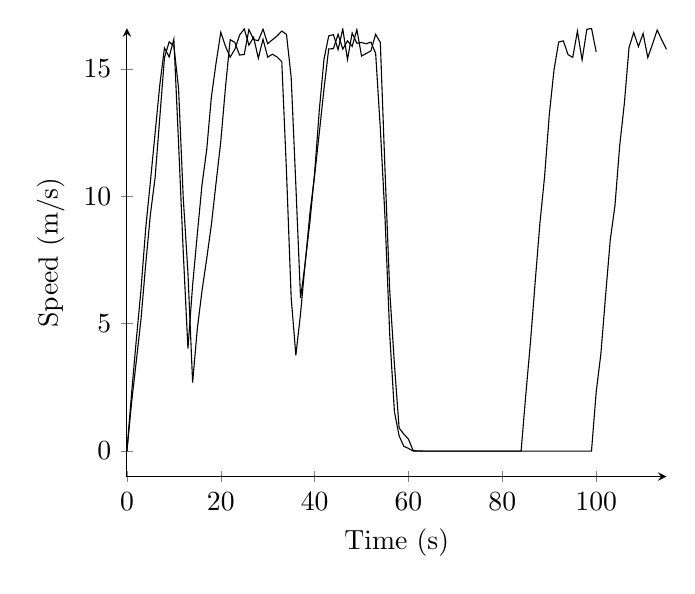
\begin{tikzpicture}
\begin{axis}[
legend style={
	anchor=west
},
axis x line=bottom,
axis y line=left,
ymin=-1,
point meta=explicit symbolic,
xlabel=Time (s),
ylabel=Speed (m/s)
]
\addplot[] coordinates {
(0, 0.0)
(1, 2.28924769326)
(2, 4.37082564866)
(3, 6.34355094458)
(4, 8.73411566165)
(5, 10.573058367)
(6, 12.4716522096)
(7, 14.3611279893)
(8, 15.8233708239)
(9, 15.471287072)
(10, 16.16557917)
(11, 12.1010938097)
(12, 7.82388430073)
(13, 4.02102297376)
(14, 6.51611162)
(15, 8.51803995029)
(16, 10.4501237752)
(17, 11.8231520447)
(18, 13.9028847759)
(19, 15.235970229)
(20, 16.4354677015)
(21, 15.8890324121)
(22, 15.460391911)
(23, 15.7719455295)
(24, 16.3234528596)
(25, 16.5707647486)
(26, 15.9316428963)
(27, 16.2380028437)
(28, 15.4177998018)
(29, 16.1635406233)
(30, 15.4613074631)
(31, 15.5764074204)
(32, 15.4686029435)
(33, 15.280803205)
(34, 10.9827677155)
(35, 6.02650071073)
(36, 3.75989515599)
(37, 5.38861945477)
(38, 7.42701642538)
(39, 8.99643731509)
(40, 10.9224178549)
(41, 13.3881508422)
(42, 15.3842817398)
(43, 16.2929289878)
(44, 16.3459788239)
(45, 15.756744761)
(46, 16.5648690809)
(47, 15.3677596975)
(48, 16.4078197293)
(49, 16.0059787251)
(50, 16.0350062724)
(51, 15.9883503199)
(52, 16.0495360099)
(53, 15.6158897307)
(54, 12.6614767091)
(55, 9.16278182974)
(56, 4.58222277776)
(57, 1.54923237715)
(58, 0.599869620279)
(59, 0.192037791967)
(60, 0.102055452704)
(61, 0.0)
(62, 0.0)
(63, 0.0)
(64, 0.0)
(65, 0.0)
(66, 0.0)
(67, 0.0)
(68, 0.0)
(69, 0.0)
(70, 0.0)
(71, 0.0)
(72, 0.0)
(73, 0.0)
(74, 0.0)
(75, 0.0)
(76, 0.0)
(77, 0.0)
(78, 0.0)
(79, 0.0)
(80, 0.0)
(81, 0.0)
(82, 0.0)
(83, 0.0)
(84, 0.0)
(85, 2.21377880458)
(86, 4.28367789689)
(87, 6.63819788577)
(88, 8.92864667985)
(89, 10.7669118128)
(90, 13.1886917033)
(91, 14.9427506584)
(92, 16.0550073752)
(93, 16.0999946468)
(94, 15.5628232855)
(95, 15.4488024147)
(96, 16.4806759034)
(97, 15.3517340339)
(98, 16.546862121)
(99, 16.5962898815)
(100, 15.667707475)
};
\addplot[] coordinates {
(0, 0.0)
(1, 1.9129509604)
(2, 3.53359989444)
(3, 5.17680118268)
(4, 7.33203553827)
(5, 9.28380112746)
(6, 10.7230726394)
(7, 13.076742471)
(8, 15.4409604878)
(9, 16.0590437951)
(10, 15.9023374586)
(11, 14.2463325608)
(12, 9.94169527128)
(13, 7.00929632751)
(14, 2.69216338119)
(15, 4.80412340553)
(16, 6.29045497398)
(17, 7.55009068471)
(18, 8.89051774143)
(19, 10.5336139354)
(20, 12.1515828974)
(21, 14.2684923747)
(22, 16.146731681)
(23, 16.0411018663)
(24, 15.5415246178)
(25, 15.5664129776)
(26, 16.5481201117)
(27, 16.1500050651)
(28, 16.1064535388)
(29, 16.5608603772)
(30, 15.9888684758)
(31, 16.1434744531)
(32, 16.2925370296)
(33, 16.4857969488)
(34, 16.3515803485)
(35, 14.675034206)
(36, 10.4233478295)
(37, 6.00115944858)
(38, 7.38546364352)
(39, 9.34858159069)
(40, 10.8230186038)
(41, 12.4987453967)
(42, 14.220058576)
(43, 15.7825445832)
(44, 15.7941047268)
(45, 16.360686332)
(46, 15.7767828641)
(47, 16.102035692)
(48, 15.8835165234)
(49, 16.542538793)
(50, 15.5059188435)
(51, 15.6063188839)
(52, 15.7075024311)
(53, 16.3595875466)
(54, 16.0370890581)
(55, 11.0139175032)
(56, 6.29822607399)
(57, 3.41178570874)
(58, 0.907085971626)
(59, 0.666657577149)
(60, 0.468068113855)
(61, 0.0164715157772)
(62, 0.00803401472455)
(63, 0.0)
(64, 0.0)
(65, 0.0)
(66, 0.0)
(67, 0.0)
(68, 0.0)
(69, 0.0)
(70, 0.0)
(71, 0.0)
(72, 0.0)
(73, 0.0)
(74, 0.0)
(75, 0.0)
(76, 0.0)
(77, 0.0)
(78, 0.0)
(79, 0.0)
(80, 0.0)
(81, 0.0)
(82, 0.0)
(83, 0.0)
(84, 0.0)
(85, 0.0)
(86, 0.0)
(87, 0.0)
(88, 0.0)
(89, 0.0)
(90, 0.0)
(91, 0.0)
(92, 0.0)
(93, 0.0)
(94, 0.0)
(95, 0.0)
(96, 0.0)
(97, 0.0)
(98, 0.0)
(99, 0.0)
(100, 2.31431862514)
(101, 3.8179840782)
(102, 6.09157453262)
(103, 8.29158702109)
(104, 9.63126861287)
(105, 11.9689060835)
(106, 13.6399704841)
(107, 15.8400485612)
(108, 16.4301891176)
(109, 15.8743815432)
(110, 16.3902995741)
(111, 15.4451811433)
(112, 15.9681985498)
(113, 16.5276055794)
(114, 16.1257917268)
(115, 15.7583096507)
};

\end{axis}
\end{tikzpicture}
\label{tik:50:12_O, 11_N, 8_N, 7_N, 7_N.-60, 5_N, 4_N, 4_N.-60, 2_V}
\caption{50 percent diving with GSC on route $12_O, 11_N, 8_N, 7_N, 7_N.-60, 5_N, 4_N, 4_N.-60, 2_V$}
\end{figure}
